\documentclass{article}\usepackage[]{graphicx}\usepackage[]{color}
%% maxwidth is the original width if it is less than linewidth
%% otherwise use linewidth (to make sure the graphics do not exceed the margin)
\makeatletter
\def\maxwidth{ %
  \ifdim\Gin@nat@width>\linewidth
    \linewidth
  \else
    \Gin@nat@width
  \fi
}
\makeatother

\definecolor{fgcolor}{rgb}{0.345, 0.345, 0.345}
\newcommand{\hlnum}[1]{\textcolor[rgb]{0.686,0.059,0.569}{#1}}%
\newcommand{\hlstr}[1]{\textcolor[rgb]{0.192,0.494,0.8}{#1}}%
\newcommand{\hlcom}[1]{\textcolor[rgb]{0.678,0.584,0.686}{\textit{#1}}}%
\newcommand{\hlopt}[1]{\textcolor[rgb]{0,0,0}{#1}}%
\newcommand{\hlstd}[1]{\textcolor[rgb]{0.345,0.345,0.345}{#1}}%
\newcommand{\hlkwa}[1]{\textcolor[rgb]{0.161,0.373,0.58}{\textbf{#1}}}%
\newcommand{\hlkwb}[1]{\textcolor[rgb]{0.69,0.353,0.396}{#1}}%
\newcommand{\hlkwc}[1]{\textcolor[rgb]{0.333,0.667,0.333}{#1}}%
\newcommand{\hlkwd}[1]{\textcolor[rgb]{0.737,0.353,0.396}{\textbf{#1}}}%

\usepackage{framed}
\makeatletter
\newenvironment{kframe}{%
 \def\at@end@of@kframe{}%
 \ifinner\ifhmode%
  \def\at@end@of@kframe{\end{minipage}}%
  \begin{minipage}{\columnwidth}%
 \fi\fi%
 \def\FrameCommand##1{\hskip\@totalleftmargin \hskip-\fboxsep
 \colorbox{shadecolor}{##1}\hskip-\fboxsep
     % There is no \\@totalrightmargin, so:
     \hskip-\linewidth \hskip-\@totalleftmargin \hskip\columnwidth}%
 \MakeFramed {\advance\hsize-\width
   \@totalleftmargin\z@ \linewidth\hsize
   \@setminipage}}%
 {\par\unskip\endMakeFramed%
 \at@end@of@kframe}
\makeatother

\definecolor{shadecolor}{rgb}{.97, .97, .97}
\definecolor{messagecolor}{rgb}{0, 0, 0}
\definecolor{warningcolor}{rgb}{1, 0, 1}
\definecolor{errorcolor}{rgb}{1, 0, 0}
\newenvironment{knitrout}{}{} % an empty environment to be redefined in TeX

\usepackage{alltt}
\IfFileExists{upquote.sty}{\usepackage{upquote}}{}
\begin{document}

\title{What is the Average Age of the Williams College Faculty?}
\author{Daishiro Nishida '18}
\maketitle

This paper investigates the average age of the Williams College faculty.\\

The average age of the Williams College faculty is 49.0 years.

\begin{knitrout}
\definecolor{shadecolor}{rgb}{0.969, 0.969, 0.969}\color{fgcolor}\begin{kframe}
\begin{verbatim}
## Mean =  49.02558 
## Standard Deviation =  12.1558
\end{verbatim}
\end{kframe}
\end{knitrout}

Here is the top of the table.\\

\begin{knitrout}
\definecolor{shadecolor}{rgb}{0.969, 0.969, 0.969}\color{fgcolor}
\begin{tabular}{l|l|r|r}
\hline
name & department & year\_of\_BA & ages\\
\hline
Donald de B. Beaver & History & 1958 & 78\\
\hline
Charles B. Dew & History & 1958 & 78\\
\hline
Eugene J. Johnson III & Art & 1959 & 77\\
\hline
Marek Demianski & Astronomy & 1962 & 74\\
\hline
Anthony J. Nicastro & Romance Languages & 1962 & 74\\
\hline
\end{tabular}


\end{knitrout}
\hfill
\\
From this it can be seen that the oldest members of the faculty are Professor Donald de B. Beaver and Professor Charles B. Dew, both in the History Department. They received their BA in the year 1958 and thus their estimated age is 78 years.\\

Now here is the bottom of the table.\\

\begin{knitrout}
\definecolor{shadecolor}{rgb}{0.969, 0.969, 0.969}\color{fgcolor}
\begin{tabular}{l|l|r|r}
\hline
name & department & year\_of\_BA & ages\\
\hline
Kevin A. Escudero & Latina/o Studies & 2009 & 27\\
\hline
Marcela Romero & Romance Languages & 2009 & 27\\
\hline
Scott D. Honecker & Physical Education & 2010 & 26\\
\hline
Qing Wang & Statistics & 2010 & 26\\
\hline
Sarah A. Mirseydi & Art & 2011 & 25\\
\hline
\end{tabular}


\end{knitrout}
\hfill
\\
The youngest member of the faculty is Professor Sarah A. Mirseydi in the Art Department, who received her BA in the year 2011 and is estimated to be 25 years old.\\

Here is a histogram.

\begin{knitrout}
\definecolor{shadecolor}{rgb}{0.969, 0.969, 0.969}\color{fgcolor}\begin{figure}[h]
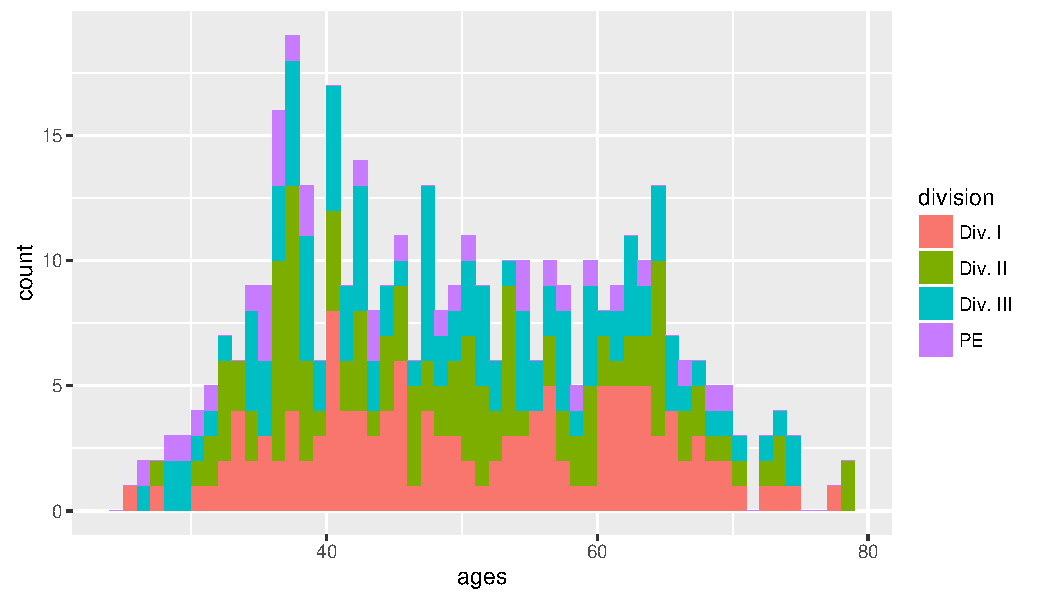
\includegraphics[width=\maxwidth]{figure/unnamed-chunk-4-1} \caption[Histogram]{Histogram}\label{fig:unnamed-chunk-4}
\end{figure}


\end{knitrout}

Now age distributions in each department.
\begin{knitrout}
\definecolor{shadecolor}{rgb}{0.969, 0.969, 0.969}\color{fgcolor}\begin{figure}[h]
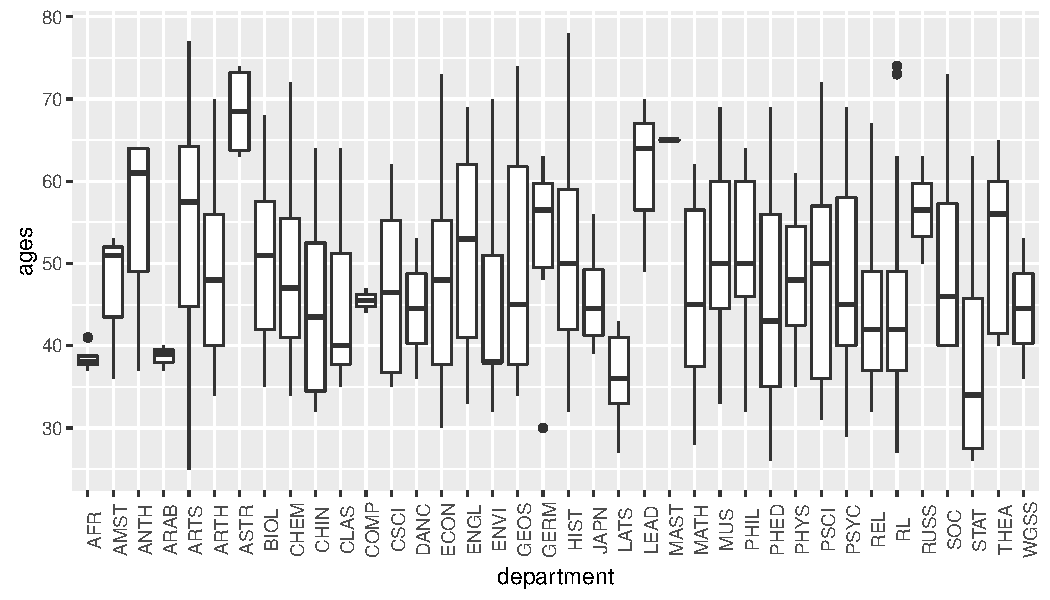
\includegraphics[width=\maxwidth]{figure/unnamed-chunk-5-1} \caption[Department]{Department}\label{fig:unnamed-chunk-5}
\end{figure}


\end{knitrout}

Finally scatter plot with last degree.
\begin{knitrout}
\definecolor{shadecolor}{rgb}{0.969, 0.969, 0.969}\color{fgcolor}\begin{figure}[h]
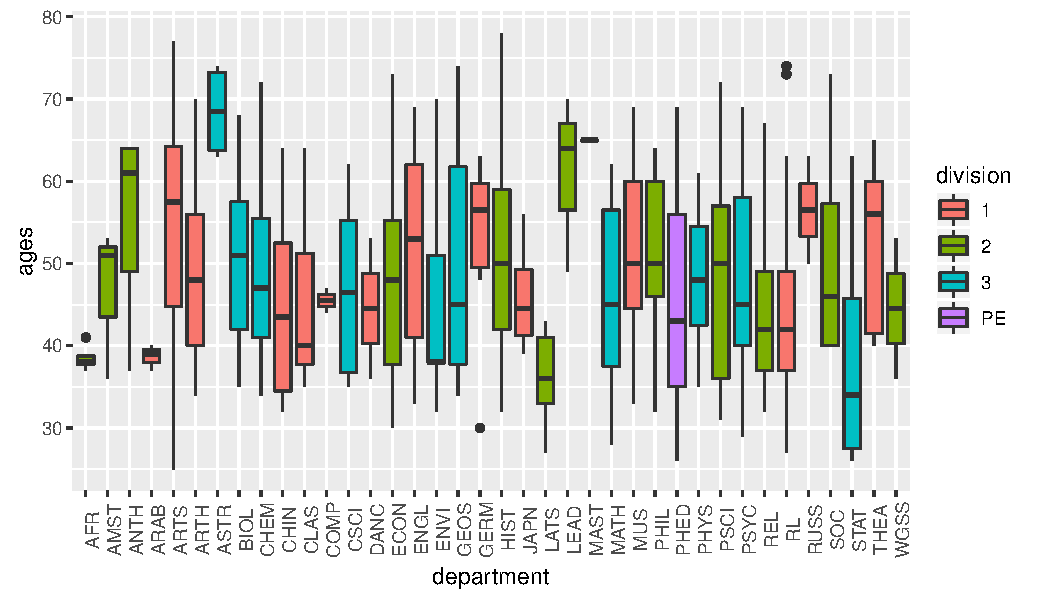
\includegraphics[width=\maxwidth]{figure/unnamed-chunk-6-1} \caption[Last degree]{Last degree}\label{fig:unnamed-chunk-6}
\end{figure}


\end{knitrout}

\end{document}
